\documentclass[11pt]{article}
\usepackage{amsmath, amssymb, amscd, amsthm, amsfonts}

\usepackage{graphicx}
\graphicspath{ {./img/} }


\usepackage{hyperref}
\usepackage{subfiles}
\usepackage{subcaption}



\oddsidemargin 0pt
\evensidemargin 0pt
\marginparwidth 40pt
\marginparsep 10pt
\topmargin -20pt
\headsep 10pt
\textheight 8.7in
\textwidth 6.65in
\linespread{1.2}

\title{Autoencoder e Sistemi Dinamici}
\author{Pietro Sillano}
%\date{11/01/2022}

\begin{document}
\maketitle
\nocite{1} 


%MAX 4 PAGINE 
%MAX 6 FIGURES
% VOLENDO INFORMAZIONI ADDIZIONALI IN APPENDICE

\section{Introduzione/Abstract}
L'idea del paper considerato consiste nello sviluppare un approccio che contemporaneamente individui un modello per un sistema dinamico e delle coordinate rappresentative del sistema.
Il primo obiettivo viene raggiunto attraverso una sparse regression in una libreria di funzioni candidate mentre il secondo viene raggiunto tramite l'utilizzo di un autoencoder tramite una riduzione di dimensionalitá del sistema.
\section{Obiettivi/Problem,question,task}
Risulta opportuna l'unione di questi due metodi in quanto non sempre i dati che vengono raccolti rappresentano la dinamica del sistema nella migliore e nella piú semplice rappresentazione possibile. 
Mentre gli autoencoder possono essere allenati individualmente per effettuare riduzioni di dimensionalitá non c'é garanzia che le coordinate intrinseche (nel latent space) individuate avranno dei modelli dinamici associati semplici e sparsi.


\section{Metodi}

\subsection{Dataset}
Un punto a favore di questo tipo di architettura é la grande quantitá di samples che é possibile generare sinteticamente e la libertá con cui é possibile manipolare e condizionare il dataset; per esempio il numero di condizioni iniziali del sistema dinamico che stiamo considerando, la possibilitá di poter studiare segnali temporali con un noise inserito ad hoc o l'intervallo temporale con cui integriamo le equazioni del moto.

\subsubsection{Lorentz}

\subsubsection{Pendolo}
In questo caso i samples del dataset considerato sono snapshot(istantanee) di un video del moto di un pendolo.

%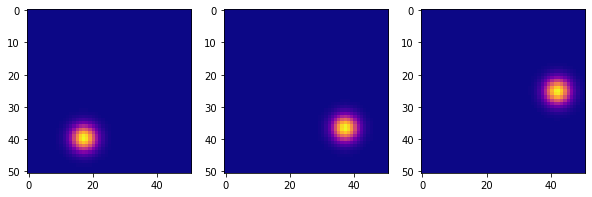
\includegraphics[width=10cm,]{pendulum_motion}
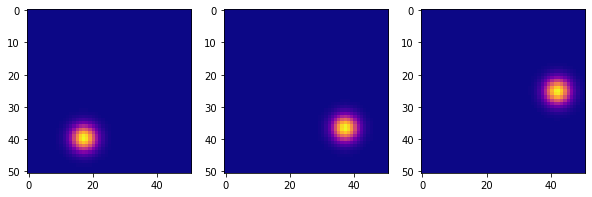
\includegraphics[width=\textwidth]{pendulum_motion}
Ricordando l'equazione del moto di un pendolo:
$$ \ddot{\theta} = \sin(\theta) $$
che posso riscrivere come un sistema di due ODE del primo ordine, ossia:

$$
\begin{cases} 
\dot{\theta} = \omega \\ 
\dot{\omega} = \sin(\theta)
\end{cases}
$$

con condizioni iniziali $\theta_0$ e $\omega_0$ scelte arbitrariamente.

Ho integrato numericamente questo sistema con un integratore RK4 (Runge-Kutta del $4^o$ ordine) ottenendo l'andamento di $\theta$ e $\omega$ nel tempo.

Successivamente per generare il video del pendolo ho generato una funzione 2d della forma di una gaussiana dipendente da $\theta(t)$:


$$G(x,y,\theta(t)) = e^{-A[(x - \cos{\theta(t)})^2 + (y - \sin{\theta(t)})^2]}$$

dove A é una costante che determina l'ampiezza della gaussiana, mentre $x$ e $y$ sono punti di una griglia $NX$ x $NY$ in cui ho valutato la funzione in ogni punto ottenendo un immagine di questo tipo:

In questo modo é possibile generare molti samples.
É importante peró variare le condizioni iniziali in modo che la rete possa avere samples del sistema in ogni punto della dinamica.

Per generare il dataset sono state usate 100 condizioni iniziali per $\theta_0$ e 100 per $\omega_0$ combinandole assieme e escludendo le condizioni iniziali per cui il pendolo non ha un attrattore "chiuso" o con un ciclo limite. Complessivamente quindi rimangono circa 5000 condizioni iniziali differenti.

\subsection{Architettura}
L'architettura presentata nel paper é stata riscritta in PyTorch.


\subsection{Loss }
Un punto principale di questa architettura é come vengono definite e usate le funzioni di costo della rete. Infatti la loss non é semplicemente la MSE loss (mean squared loss) tra l'input x dell' autoencoder e la ricostruzione $\tilde{x}$ in output. Vengono aggiunti alcuni termini che garantiscono oltre alla ricostruzione dell'input, anche la ricostruzione delle derivate temporali $\dot{x}$ e $\dot{z}$ e infine é presente anche un termine di regolarizzazione L1 sui coefficienti $\xi $ in modo da promuovere la sparsity di quest'ultimi.
\newline

\begin{itemize}
\item $L_{recon} = \|x - \tilde{x}|_2^2 $ questa misura quanto bene l'autoencoder riesce a ricostruire l'input x.
\item $L_{dz} = \|\dot{z} - \theta(z)\xi\|_2^2 $ vedi paper cosa dice
\item $L_{dx} = \|\dot{x} - \dot{\tilde{x}}\|_2^2 $ misura quanto le predizioni di Sindy ossia $\dot{\tilde{x}}$ possano essere usate per ricostruire l'input originale $\dot{x}$
\item $L_{reg} = \|{\xi}\|_1 $ é una regolarizzazione L1 che promuove la sparsity dei coefficienti $\xi$ che coincide con i nostri obiettivi perché noi vorremmo scoprire modelli parsimoniosi ossia con il minor numero di parametri possibile.
\end{itemize}
Per cui combinando insieme i quattro termini di loss insieme ai relativi iperparametri la loss finale é la seguente: 
$$L_{tot} = L_{recon} + \lambda_1L_{dx} + \lambda_2L_{dz} + \lambda_3L_{reg} $$
In queste loss compaiono delle derivate temporali di alcune grandezze: $\dot{x}$ assumiamo di poterla calcolare a partire dai dati di input mentre $\dot{z}$ e $\dot{\tilde{x}}$ non possiamo calcolarle tramite backpropagation della rete.
Dobbiamo quindi trovare un metodo per esprimere tali grandezze in funzione delle grandezze note.

x = input, y = output della rete, $z = w^{\top}x + b$ , $f(z) $ funzione di attivazione differenziabile, $a_{l}(z) = f(z_l)$ attivazione del layer l, l = layer l  della rete e m = numero di layer nella rete
$$ 
\frac{dy}{dt} =
\frac{dy}{dx}\frac{dx}{dt} =
\frac{dx}{dt}\prod_{l=0}^{m-1} \frac{da_l}{dx} =
\frac{dx}{dt}\prod_{l=0}^{m-1} \frac{df(z_l)}{dx} =
\dot{x}\prod_{l=0}^{m-1} \frac{df(z_l)}{dz_l}\frac{dz_l}{dx} = 
\dot{x}\prod_{l=0}^{m-1} \frac{df(z_l)}{dz_l}w_l^{\top} 
$$

Applicando questa regola con $y = \dot{z} $ é possibile calcolarla a partire da $\dot{x}$ e allo stesso modo se $y = \dot{\tilde{x}}$ a partire da $\dot{\tilde{z}}$ quest ultima ricavata con Sindy $\dot{\tilde{z}} = \theta(z)\xi$

\subsection{Dettagli Training}
Batch size = 1024
Funzione di attivazione $f$ = ReLU o Sigmoide

\section{Risultati}
plot con le loss standard

plot con le traiettorie predette a confronto con quelle originali


\section{Conclusioni e possibili sviluppi futuri}
Estendere ad altri sistemi dinamici
modificare e rendere piu deep l architettura



\bibliographystyle{plain}
\bibliography{bibliography.bib}

\section{Codice}
É possibile trovare l'implementazione del codice su \url{https://github.com/pietro-sillano/SindyPendulum}

\end{document}
